\documentclass[t]{beamer}

% --- Packages ---
\usepackage{tikz}
\usetikzlibrary{patterns, arrows.meta, decorations.markings, positioning, shapes.geometric}
\usepackage{graphicx}
\graphicspath{{inference_results/annotated/}{evaluation_plots/}}
\usepackage{booktabs}
\usepackage{natbib}
\usepackage{amsmath}
\usepackage{amssymb}
\usepackage{eso-pic}
% --- Theme ---
\usetheme{Madrid}

% --- Colors ---
\definecolor{MyOrange}{RGB}{230, 85, 10}
\definecolor{NavDarkBlue}{RGB}{15, 32, 67}
\definecolor{CodeBg}{RGB}{245, 245, 245}

\usecolortheme[named=MyOrange]{structure}

\setbeamercolor{palette primary}{bg=MyOrange,fg=white}
\setbeamercolor{palette secondary}{bg=MyOrange!85!black,fg=white}
\setbeamercolor{palette tertiary}{bg=MyOrange!70!black,fg=white}
\setbeamercolor{titlelike}{parent=palette primary}
\setbeamercolor{block title}{bg=MyOrange!90!black,fg=white}
\setbeamercolor{block body}{bg=MyOrange!5!white,fg=black}

% --- Fonts & Formatting ---
\setbeamerfont{caption}{size=\footnotesize}
\setbeamertemplate{navigation symbols}{}
\setbeamertemplate{footline}[frame number]

% --- Title Info ---
\title[Face Recognition In The Wild]{FACE RECOGNITION IN THE WILD: 4-PHASE ARCHITECTURE}
\subtitle{Faster RCNN, IResNet-100, Anet, \& GCN-Clustering Pipeline}
\author[Face Recognition Team]{Akshat Porwal (NA22B025), Suharsh Kumar (BE22B037)}

\date{\today}

\begin{document}

% ==============================================================================
% Title Slide
% ==============================================================================

\begin{frame}
    \titlepage

\end{frame}


% ==============================================================================
% Table of Contents
% ==============================================================================
\begin{frame}{Table of Contents}
    \tableofcontents
\end{frame}
\usebackgroundtemplate{}
% ==============================================================================
% SECTION: ARCHITECTURE OVERVIEW
% ==============================================================================
\section{Architecture Overview}

\begin{frame}{Overall Architecture Phases}
    \begin{block}{The 4-Phase Pipeline}
        \begin{itemize}
            \item \textbf{Phase 0}: Fine-tune Faster RCNN trained on COCO dataset for object detection.
            \item \textbf{Phase 1}: Feature extraction with IResNet-100, Curricular Loss, and BroadFace.
            \item \textbf{Phase 2}: Anet using multiple kernel sizes to capture global and local features.
            \item \textbf{Phase 3}: Unlabelled image pseudo-labeling, Graph construction, and GCN Clustering.
        \end{itemize}
    \end{block}

    \vspace{0.5cm}

    \begin{center}
    \resizebox{0.9\textwidth}{!}{
    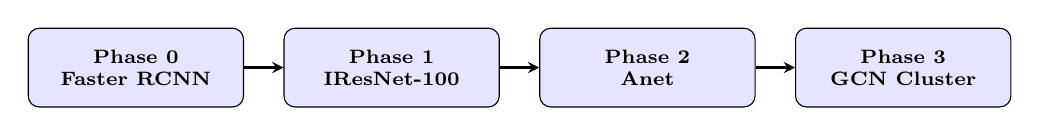
\begin{tikzpicture}[node distance=1.2cm, auto, >=stealth]
        \tikzstyle{block} = [rectangle, draw, fill=blue!10, text width=2.5cm, text centered, rounded corners, minimum height=1cm, font=\scriptsize\bfseries]

        \node [block] (p0) {Phase 0\\Faster RCNN};
        \node [block, right=0.5cm of p0] (p1) {Phase 1\\IResNet-100};
        \node [block, right=0.5cm of p1] (p2) {Phase 2\\Anet};
        \node [block, right=0.5cm of p2] (p3) {Phase 3\\GCN Cluster};

        \draw [->, thick] (p0) -- (p1);
        \draw [->, thick] (p1) -- (p2);
        \draw [->, thick] (p2) -- (p3);
    \end{tikzpicture}
    }
    \end{center}
\end{frame}

% ==============================================================================
% SECTION: PHASE 0 - FASTER RCNN
% ==============================================================================
\section{Phase 0: Faster R-CNN Fine-Tuning}

\begin{frame}[allowframebreaks]{Phase 0: Finetuning Faster RCNN}
    \begin{block}{1. Fine-Tuning & Backbone}
        \begin{itemize}
            \item \textbf{Transfer Learning}: Fine-tuning a pre-trained Faster R-CNN (originally trained on COCO's 81 object classes).
            \item \textbf{Model Adaptation}: Replaced the final classification head to specialize in a 2-class detection task (Face vs. Background).
            \item \textbf{Backbone (ResNet-50 + FPN)}: Extracts multi-scale feature maps (P2--P6) to maintain robust detection across varying face scales.
        \end{itemize}
    \end{block}
\end{frame}
    \begin{figure}
    \centering
    \includegraphics[width=0.6\linewidth]{image1.png}
    \caption{Source: https://arxiv.org/pdf/1405.0312}
    \label{fig:placeholder}
\end{figure}



\begin{frame}{Phase 0: Faster RCNN}
    \begin{block}{2. Region Proposal Network (RPN), IoU & Sampling}
        \begin{itemize}
            \item \textbf{Anchors}: Generated across FPN scales (16x16 to 256x256).
            \item \textbf{Matching (IoU)}: Anchors with IoU \(>\) 0.7 are positive; IoU \(< \)0.3 are negative.
            \item \textbf{Sampling}: A fixed ratio (1:3) of positive/negative samples is used to form a balanced training batch.
            \item \textbf{Training Goal}: These samples train the RPN to perform objectness classification and BBox regression.
            \item \textbf{Downstream usage}: The refined proposals (RPN-adjusted bounding boxes with associated objectness scores) are passed to the \textbf{RoI Heads} for final classification (face/background) and precise coordinate refinement.
        \end{itemize}
    \end{block}
    \framebreak



  \end{frame}
  \begin{frame}
   \begin{figure}
    \centering
    \includegraphics[width=0.8\linewidth]{image.png}
    \caption{Source: https://brunofuga.adv.br/?s=faster-r-cnn-explained-for-object-detection-tasks-paperspace-cc-zzkKmWIk}

    \label{fig:placeholder}
\end{figure}
     \begin{block}{3. RoI Align & Detection Head}
        \begin{itemize}
            \item \textbf{RoI Align}: Maps variable-sized RPN proposals into a fixed 7$\times$7 spatial feature map using bilinear interpolation, effectively avoiding the quantization misalignment errors inherent in traditional RoI Pooling.


        \end{itemize}
    \end{block}




\end{frame}





% ==============================================================================
% SECTION: PHASE 1 - FEATURE EXTRACTION
% ==============================================================================
\section{Phase 1: Feature Extraction (IResNet-100)}

\begin{frame}[allowframebreaks]{Phase 1: IResNet-100, Curricular Loss, & BroadFace}
    \begin{block}{IResNet-100 Backbone}
        \begin{itemize}
            \item \textbf{Embedding Generation}: Transforms input face crops into a discriminative 512-D L2-normalized embedding vector.
            \item \textbf{Identity Preservation}: Deep feature extractor ensures robust identity representation via improved gradient flow.
            \item \textbf{Embedding Manifold}: Maps faces to a space where intra-class distance is minimized and inter-class distance is maximized.
        \end{itemize}
    \end{block}

    \begin{block}{Curricular Learning}
        \begin{itemize}
            \item Protocol: $\mathcal{L}_{\text{Curricular}} = -\log \frac{e^{s(\cos\theta_{y_i} - m(t))}}{e^{s(\cos\theta_{y_i} - m(t))} + \sum_{j \neq y_i} e^{s \cdot N(t, j) \cdot \cos\theta_j}}$
            \item Strategy: Starts with easy samples, gradually introducing harder ones using parameter $t$ to control learning pace and margin $m(t)$.
        \end{itemize}
    \end{block}
    \framebreak
    \begin{block}{BroadFace: Handling Long-Tail Distributions}
        \begin{itemize}
            \item \textbf{Mechanism}: Maintains a DDP-safe, detached memory queue of past face embeddings, labels, and classifier proxies (weights).
            \item \textbf{Drift Compensation}: Adjusts stored features for classifier weight updates to ensure stable training across iterations.
            \item \textbf{Loss Computation}: Combines current batch loss with compensated queue loss, preventing backpropagation of stale representations into the backbone.
            \item \textbf{Benefit}: Boosts representation for under-represented "long-tail" identities by effectively extending training context.
        \end{itemize}
    \end{block}
\end{frame}

% ==============================================================================
% SECTION: PHASE 2 - ANET
% ==============================================================================
\section{Phase 2: Anet Feature Refinement}

\begin{frame}[allowframebreaks]{Phase 2: Anet - Dual-Path Attribute Parsing}
    \begin{block}{1. Dual-Path Architecture}
        \begin{itemize}
            \item \textbf{Global Path}: Processes full aligned face crop (112x112) to capture global facial structure $\rightarrow$ 128x7x7 feature map.
            \item \textbf{Landmark-Guided Local Path}: Dynamically extracts facial patches (eyes, nose, mouth) based on detected landmarks to focus on potentially occluded regions $\rightarrow$ 64x7x7 feature map.
        \end{itemize}
    \end{block}

    \begin{block}{2. Feature Fusion}
        \begin{itemize}
            \item \textbf{Concatenation}: Merges Global and Local feature maps (192 channels total).
            \item \textbf{Fusion Conv}: Refines concatenated features to a unified 256x7x7 spatial representation.
        \end{itemize}
    \end{block}
    \framebreak

    \begin{block}{3. Multi-Task Output}
        \begin{itemize}
            \item \textbf{40-Attribute Classifier}: Maps fused features to 40 binary facial attributes (e.g., Eyeglasses, Young, Wearing\_Hat) using a fully connected head.
            \item \textbf{Spatial Occlusion Attention}: Generates a 1x7x7 sigmoid mask ($M_{spatial}$) highlighting regions with low feature confidence.
            \item \textbf{Occlusion Logic}: Determines \texttt{is\_occluded} status based on attribute indicators (Glasses/Hat) and low spatial attention weights.
        \end{itemize}
    \end{block}
\end{frame}

% ==============================================================================
% SECTION: PHASE 3 - GCN CLUSTERING
% ==============================================================================
\section{Phase 3: Unlabelled Graph Clustering via GCN}

\begin{frame}[allowframebreaks]{Phase 3: GCN Clustering}
    \begin{block}{Theoretical Foundation \& Notations}
        \begin{itemize}
            \item \textbf{Symbols}:
                \begin{itemize}

                    \item $H^{(l)}$: Feature matrix at layer $l$ of dimension $(N, d)$.
                    \item $A$: Adjacency matrix (KNN).

                    \item $D$: Diagonal Degree matrix of $\tilde{A}$ ($D_{ii} = \sum_{j} \tilde{A}_{ij}$).
                    \item $\hat{A} = \tilde{D}^{-1/2} \tilde{A} \tilde{D}^{-1/2}$: Normalized Adjacency for stability.

                \end{itemize}
            \item \textbf{GCN Operation}: $H^{(l+1)} = \text{PReLU}(\hat{A} H^{(l)} W^{(l)})$.
        \end{itemize}
    \end{block}

    \begin{block}{1. Graph Construction (Build)}
        \begin{itemize}
            \item \textbf{KNN Graph}: Computes all-pair cosine similarity, keeps top-$k$ connections.
            \item \textbf{Symmetric Normalization}: $\hat{A} = \tilde{D}^{-1/2} \tilde{A} \tilde{D}^{-1/2}$, where $\tilde{A} = A+I$. This ensures stability across varying node degrees.
        \end{itemize}
    \end{block}

    \begin{block}{2. Feature Propagation (3-Layer GCN)}
        \begin{itemize}
            \item \textbf{Inputs}:
                \begin{itemize}
                    \item Node Features ($H^{(0)}$): 512-D IResNet-100 embeddings.
                    \item Normalized Adjacency ($\hat{A}$): Connectivity graph structure.
                \end{itemize}
            \item \textbf{Operation}: $H^{(l+1)} = \text{PReLU}(\hat{A} H^{(l)} W^{(l)})$.
            \item \textbf{Residual Connection}: $h_{out} = \text{GCN}_3(h_2) + h_1$ to mitigate over-smoothing and vanishing gradients.
        \end{itemize}
    \end{block}

    \begin{block}{3. Link Prediction & Clustering}
        \begin{itemize}
            \item \textbf{Output}: Pairwise Edge Probability $P(edge_{ij}) \in [0, 1]$ using a 4-Way Edge Interaction MLP: $[h_i, h_j, |h_i-h_j|, h_i \odot h_j]$.
            \item \textbf{Refined Graph}: Edges $A^{cluster}_{ij} = 1$ if $P(edge_{ij}) > \tau$.
            \item \textbf{Pseudo-Labeling}: Connected Components (BFS) on $A^{cluster}$ assign globally unique IDs to high-confidence node clusters.
        \end{itemize}
    \end{block}

    \begin{block}{4. Clustering Mechanism: Refining Identity Labels}
        \begin{itemize}
            \item \textbf{Identity Refinement}: Each component is assigned a coherent pseudo-label, which acts as a refined identity label, effectively expanding and correcting the identity space established in Phase 1.
        \end{itemize}
    \end{block}
\end{frame}

% ==============================================================================
% SECTION: BENCHMARKS
% ==============================================================================
\section{Benchmarks}
\begin{frame}{Training Loss Curve}
    \begin{figure}
        \centering
        \includegraphics[width=0.85\linewidth]{training_loss_curve.png}
        \caption{Phase 0 Faster R-CNN Training Loss Curve}
    \end{figure}
\end{frame}
\begin{frame}{Metric Definitions}
    \begin{block}{Detection Metrics}
        \begin{itemize}
            \item \textbf{GT (Ground Truth)}: Total actual faces annotated in the dataset.
            \item \textbf{Preds (Predictions)}: Total face bounding boxes detected by the model.
            \item \textbf{Prec. (Precision)}: $\frac{TP}{TP + FP}$. Accuracy of detections (low false alarms).
            \item \textbf{Recall}: $\frac{TP}{TP + FN}$. Coverage of detections (low missed faces).
            \item \textbf{F1}: Harmonic mean of Precision and Recall; provides a balanced performance score.
            \item \textbf{AP@0.5}: Average Precision at 50\% IoU overlap. Measures overall ranking and localization quality.
        \end{itemize}
    \end{block}
    \vspace{0.2cm}
    \begin{block}{Abbreviations}
        $TP$ = True Positives (Correct), $FP$ = False Positives (False alarm), $FN$ = False Negatives (Missed face).
    \end{block}
\end{frame}

\begin{frame}{Performance Benchmarks}
    \begin{table}
        \centering
        \caption{Localization Metrics across Evaluated Datasets}
        \label{tab:benchmarks}
        \resizebox{\textwidth}{!}{
        \begin{tabular}{lrrrrrrr}
            \toprule
            \textbf{Dataset} & \textbf{Images} & \textbf{GT} & \textbf{Preds} & \textbf{Prec.} & \textbf{Recall} & \textbf{F1} & \textbf{AP@0.5} \\
            \midrule
            widerface & 3226 & 39697 & 17560 & 80.18\% & 35.47\% & 49.18\% & 34.49\% \\
            ufdd & 6424 & 10895 & 11113 & 45.57\% & 46.48\% & 46.02\% & 40.59\% \\
            afw & 205 & 468 & 630 & 72.86\% & 98.08\% & 83.61\% & 97.63\% \\
            \midrule
            \textbf{Aggregate} & - & - & - & \textbf{66.89\%} & \textbf{38.39\%} & \textbf{48.78\%} & \textbf{57.57\%} \\
            \bottomrule
        \end{tabular}
        }
    \end{table}
    \vspace{0.5cm}
    \begin{block}{Note}
        Metrics are based on localization (face detection) accuracy. Darkface dataset excluded due to lack of ground truth.
    \end{block}
\end{frame}
\begin{frame}{Test Result: Outdoor Premiere}
    \centering
    \includegraphics[width=0.9\linewidth]{group_01_outdoor_premiere.jpg}
\end{frame}
\begin{frame}{Test Result: Evening Gathering}
    \centering
    \includegraphics[width=0.9\linewidth]{group_02_evening_gathering.jpg}
\end{frame}
\begin{frame}{Test Result: Indoor Meeting}
    \centering
    \includegraphics[width=0.9\linewidth]{group_03_indoor_meeting.jpg}
\end{frame}
\begin{frame}{Test Result: Public Event}
    \centering
    \includegraphics[width=0.9\linewidth]{group_04_public_event.jpg}
\end{frame}
\begin{frame}{Test Result: Sidelight Poses}
    \centering
    \includegraphics[width=0.9\linewidth]{group_05_sidelight_poses.jpg}
\end{frame}
\begin{frame}{Test Result: Warm/Cool Light}
    \centering
    \includegraphics[width=0.9\linewidth]{group_06_warm_cool_light.jpg}
\end{frame}
\begin{frame}{Test Result: Backlight Meeting}
    \centering
    \includegraphics[width=0.9\linewidth]{group_07_backlight_meeting.jpg}
\end{frame}
\begin{frame}{Test Result: Harsh Sun Poses}
    \centering
    \includegraphics[width=0.9\linewidth]{group_08_harsh_sun_poses.jpg}
\end{frame}
\begin{frame}{Test Result: Stadium Gathering}
    \centering
    \includegraphics[width=0.9\linewidth]{group_09_stadium_gathering.jpg}
\end{frame}
\begin{frame}{Test Result: Festival Crowd}
    \centering
    \includegraphics[width=0.9\linewidth]{group_10_festival_crowd.jpg}
\end{frame}
\begin{frame}{Test Result: Reception Backlight}
    \centering
    \includegraphics[width=0.9\linewidth]{group_11_reception_backlight.jpg}
\end{frame}
\begin{frame}{Test Result: Park Gathering}
    \centering
    \includegraphics[width=0.9\linewidth]{group_12_park_gathering.jpg}
\end{frame}
\begin{frame}{Test Result: Celebration Crowd}
    \centering
    \includegraphics[width=0.9\linewidth]{group_13_celebration_crowd.jpg}
\end{frame}
\begin{frame}{Test Result: Awards Arrival}
    \centering
    \includegraphics[width=0.9\linewidth]{group_14_awards_arrival.jpg}
\end{frame}
\begin{frame}{Test Result: Crowded Meeting}
    \centering
    \includegraphics[width=0.9\linewidth]{group_15_crowded_meeting.jpg}
\end{frame}
\begin{frame}{Test Result: Image 1}
    \centering
    \includegraphics[width=0.9\linewidth]{img_1.png}
\end{frame}
\begin{frame}{Test Result: Image 2}
    \centering
    \includegraphics[width=0.9\linewidth]{img_2.jpg}
\end{frame}
\begin{frame}{Test Result: Image 5}
    \centering
    \includegraphics[width=0.9\linewidth]{img_5.jpg}
\end{frame}
\begin{frame}{Test Result: Modi}
    \centering
    \includegraphics[width=0.9\linewidth]{modi.jpeg}
\end{frame}

\begin{frame}[allowframebreaks]{Inference Pipeline: From Image to Identity}


    \begin{block}{1. Processing Flow (Forward Pass)}
        \begin{itemize}
            \item \textbf{Phase 0 (Detection)}: `self.detector` identifies face bounding boxes and landmarks.
            \item \textbf{Cropping & Alignment}: Extracts and aligns each detected face crop. Optional \textbf{Frontalization} corrects extreme poses.
            \item \textbf{Phase 1 (Embedding)}: `self.backbone` (e.g., IResNet-100) generates the 512-D identity embedding.
            \item \textbf{Phase 2 (Attributes)}: `self.attribute\_parser` predicts occlusion status and facial attributes using the crop.
            \item \textbf{Identity Classification}: `self.ddrc\_classifier` compares the embedding against the enrolled gallery.
        \end{itemize}
    \end{block}

    \begin{block}{4. Output \& Visualization}
        \begin{itemize}
            \item \textbf{JSON Output}: Saves predictions (boxes, identity, scores) in JSONL format for downstream tasks.
            \item \textbf{Annotation}: Draws bounding boxes on images. Green for identified faces, red for unknown, including confidence scores.
        \end{itemize}
    \end{block}
\end{frame}


% ==============================================================================
% Conclusion Slide
% ==============================================================================
\begin{frame}
    \centering
    \vfill
    \Huge \textcolor{MyOrange}{\textbf{Thank You}} \\
    \vspace{0.5cm}
    \Large \textbf{Questions \& Discussion}
    \vfill
\end{frame}

\end{document}
